\documentclass[10pt,twocolumn]{article}

\usepackage[margin=0.75in]{geometry}
\usepackage{amsmath,amssymb,amsfonts}
\usepackage{graphicx}
\usepackage{booktabs}
\usepackage{hyperref}
\usepackage{microtype}
\usepackage{cite}
\usepackage{color}
\usepackage{xcolor}

\hypersetup{
    colorlinks=true,
    linkcolor=blue!70!black,
    citecolor=blue!70!black,
    urlcolor=blue!70!black
}

\title{\textbf{ConnectomePrune: Attention-Protective Non-Uniform Sparsification for Compact Language Models}}

\author{
  \textbf{R\"uzgar Vatansever} \\
  Independent Researcher \\
  \c{S}ehit \"O\u{g}retmen Necmeddin Kuyucu Anadolu Lisesi, Gebze, Kocaeli, Turkey \\
  \texttt{rzvatansevertr@gmail.com} \quad $|$ \quad ORCID: 0009-0004-9477-8422
}

\date{}

\begin{document}

\maketitle

\begin{abstract}
Deploying compact foundation language models on resource-constrained hardware requires parameter reduction without destabilizing multi-head attention routing. While empirical weight-activation pruning (e.g., Wanda) preserves magnitude outliers, standard frameworks enforce uniform sparsity across all linear projections, disproportionately degrading fragile multi-head self-attention mechanisms. Motivated by structural heterogeneity in biological connectomics and homeostatic synaptic scaling, we present \textbf{ConnectomePrune-LLM}. Our framework introduces: (1) \textit{Attention-Protective Budget Allocation}, a closed-form iso-sparsity formulation that shields high-saliency attention projections while shifting sparsity onto feed-forward MLP blocks ($\alpha_{\text{attn}} = 18.75\%, \alpha_{\text{mlp}} = 28.75\%$ on LLaMA-3.2-1B, achieving a $27.03\%$ theoretical target and $27.10\%$ empirical reduction); (2) \textit{Output-Selective Homeostatic Scaling} ($\gamma = 1/\sqrt{\rho}$), applied strictly to linear projection outputs ($W_o$ and $W_{\text{down}}$) while leaving internal query/key/gate projections unscaled to prevent temperature sharpening; and (3) \textit{ConnectomeSculptor}, an offline in-place safetensor carving tool requiring $< 3.5$ GB host RAM during pruning. On Meta LLaMA-3.2-1B across full WikiText-2 evaluation (ctx 512 / 2k), ConnectomePrune achieves 11.48 perplexity (near dense 11.24), significantly outperforming uniform Wanda (12.85) and performing on par with depth-search methods like OWL (11.84, with scaling 11.56) without requiring layer-depth hyperparameter tuning. On 50 algorithmic Python functions, ConnectomePrune preserves 100.0\% syntax validity (95\% Wilson CI: [92.9\%, 100.0\%]) compared to 80.0\% for Wanda ([67.0\%, 88.8\%]). At high sparsity (40\%), ConnectomePrune maintains a 10.55 PPL advantage over Wanda (119.03 vs. 129.58). Cross-model evaluation on Qwen2.5-1.5B confirms consistent attention fragility across two model families. Reproducibility code is available at \url{https://github.com/ruzgar1923/connectome-prune-llm}.
\end{abstract}

\section{Introduction}

Deploying modern large language models (LLMs) on resource-constrained consumer devices, mobile processors, and robotics requires substantial parameter reduction \cite{dubey2024llama}. While post-training quantization (PTQ) reduces numerical precision from FP16 to INT4/INT8, unstructured and structured pruning directly eliminate synaptic weights, reducing model parameter footprint \cite{sun2023wanda, frantar2023sparsegpt}.

Early pruning methods evaluated parameter importance solely based on weight magnitude ($|W_{ij}|$), which causes catastrophic representation collapse in LLMs due to the destruction of emergent activation outliers \cite{sun2023wanda}. To address this, Wanda (Pruning by Weights and Activations) introduced an input-channel-norm weighted saliency metric:
\begin{equation}
S_{ij} = |W_{ij}| \cdot \|X_j\|_2
\end{equation}
which preserves parameters that multiply high-magnitude activation channels. However, standard post-training pruning frameworks apply a uniform sparsity target across all transformer layers and sub-modules. In compact models (e.g., 1B to 3B parameters), parameters are structurally partitioned between Multi-Head Attention (MHA) routing projections and Feed-Forward Network (MLP) blocks. In LLaMA-3.2-1B, attention projections account for only 17.2\% of linear parameters, while MLP blocks comprise 82.8\% \cite{dubey2024llama}. 

Applying uniform sparsity across both modules treats attention routing channels identically to feed-forward associative memories. However, connectomic mapping of biological nervous systems reveals that anatomical wiring diagrams are fundamentally non-uniform: high-centrality hub pathways exhibit distinct structural density compared to modular sub-circuits \cite{dorkenwald2024neuronal, schlegel2024whole}. Furthermore, biological neural circuits maintain firing rate stability across continuous synaptic remodeling via homeostatic synaptic scaling \cite{turrigiano2008self}.

Motivated by these principles, we develop \textbf{ConnectomePrune-LLM}, an attention-protective, homeostatically scaled sparsification framework. Our contributions are:
\begin{enumerate}
    \item \textbf{Iso-Sparsity Attention Protection:} We parameterize layer-wise sparsity along a strict global iso-sparsity curve, assigning protective budgets to attention projections ($\alpha_{\text{attn}} = 18.75\%$) while absorbing compensatory sparsity in MLP blocks ($\alpha_{\text{mlp}} = 28.75\%$), targeting $27.03\%$ theoretical and achieving $27.10\%$ empirical reduction.
    \item \textbf{Output-Selective Homeostatic Scaling:} We introduce variance-restoring scaling $\gamma = 1/\sqrt{\rho}$ applied strictly to projection outputs ($W_o$ and $W_{\text{down}}$), showing that bypassing internal projections ($W_q, W_k, W_{\text{gate}}$) avoids softmax temperature distortion.
    \item \textbf{Mechanistic Saliency Analysis:} We analyze layer-wise saliency density across all 16 layers of LLaMA-3.2-1B, showing that attention projections exhibit $1.3\times$ to $2.28\times$ higher activation-weighted density than MLP blocks across the network.
    \item \textbf{High-Sparsity Resilience \& Cross-Model Validation:} We demonstrate that ConnectomePrune prevents attention collapse at 40\% and 50\% sparsity, outperforming Wanda by 10.55 PPL at 40\%, and validate architectural behavior on Qwen2.5-1.5B (28 layers).
    \item \textbf{Evaluation with OWL:} We evaluate the integration of intra-layer attention protection into depth-dependent pruning (OWL), achieving a 4.43 PPL improvement over baseline OWL (105.42 $\to$ 100.99).
\end{enumerate}

\section{Related Work}

\textbf{Post-Training Sparsification:} SparseGPT \cite{frantar2023sparsegpt} formulated pruning as a generalized layer-wise regression problem using second-order Hessian approximations, enabling 50\% unstructured sparsity with minimal reconstruction loss. Wanda \cite{sun2023wanda} showed that multiplying absolute weight magnitude by input channel $L_2$ norms achieves competitive perplexity without requiring costly Hessian inversions. 

\textbf{Non-Uniform Budgeting:} OWL (Outlier Weighed Layerwise Sparsity) \cite{yin2024owl} observed that outlier distribution varies across depth, dynamically allocating layer-wise sparsity based on activation outlier ratios. BESA (Balanced Sparsity Allocation) \cite{besa2024} and AlphaPruning \cite{alphapruning2024} formulated sensitivity sweeps across projection matrices using gradient-free search. SliceGPT \cite{ashkboos2024slicegpt} and ShortGPT \cite{men2024shortgpt} explored structural block and layer pruning, but require retraining or introduce discrete capacity drops. ConnectomePrune provides an orthogonal, closed-form intra-layer budget allocation that complements both Wanda and OWL without requiring layer-depth search.

\section{Methodology}

\subsection{Parameter Partitioning \& Saliency Formulation}
Given a transformer layer $l$, the forward pass computes:
\begin{align}
\text{Attn}(X) &= \text{Softmax}\left(\frac{X W_q (X W_k)^T}{\sqrt{d_k}}\right) X W_v W_o \\
\text{MLP}(H) &= \left(\text{SiLU}(H W_{\text{gate}}) \odot H W_{\text{up}}\right) W_{\text{down}}
\end{align}
Linear parameters are partitioned into attention routing matrices $\mathcal{W}_{\text{attn}} = \{W_q, W_k, W_v, W_o\}$ and feed-forward matrices $\mathcal{W}_{\text{mlp}} = \{W_{\text{gate}}, W_{\text{up}}, W_{\text{down}}\}$.

Input activation norms are accumulated across calibration sequences sampled from C4 \cite{sun2023wanda}:
\begin{equation}
\|X_j\|_2 = \sqrt{\sum_{t=1}^{T} X_{t,j}^2}
\end{equation}
The salience matrix for linear projection $W \in \mathbb{R}^{d_{\text{out}} \times d_{\text{in}}}$ is evaluated via Hadamard product:
\begin{equation}
S = |W| \odot \left(\mathbf{1}_{d_{\text{out}}} \otimes \|X\|_2^T\right)
\end{equation}

\subsection{Iso-Sparsity Attention Budgeting}
To maintain a theoretical target linear reduction $S_{\text{target}} = 27.03\%$, we define an attention protection factor $\kappa \in [0.60, 0.85]$. The attention sparsity is defined as $\alpha_{\text{attn}} = \kappa \cdot S_0$ ($S_0 = 0.25$). To guarantee exact global parameter conservation, MLP sparsity is constrained along the iso-sparsity manifold:
\begin{equation}
\alpha_{\text{mlp}} = \frac{S_{\text{target}} \cdot N_{\text{total}} - \alpha_{\text{attn}} \cdot N_{\text{attn}}}{N_{\text{mlp}}}
\end{equation}
For LLaMA-3.2-1B ($N_{\text{attn}} = 167.77\text{M}, N_{\text{mlp}} = 805.31\text{M}$), sweeping $\kappa \in \{0.60, 0.70, 0.75, 0.80, 0.85\}$ on the C4 validation split yielded validation perplexities of 11.62, 11.53, \textbf{11.45 (optimal at $\kappa = 0.75$)}, 11.58, and 11.74 respectively, demonstrating a distinct U-shaped minimum at $\alpha_{\text{attn}} = 0.1875$ (18.75\%) and $\alpha_{\text{mlp}} = 0.2875$ (28.75\%), pruning theoretically $262,982,861$ weights ($27.03\%$). Empirically, strict thresholding in PyTorch zeros out tied values at the boundary across 112 weight matrices, yielding $263,672,581$ pruned weights ($27.10\%$, a minor 0.07\% boundary deviation).

\subsection{Output-Selective Homeostatic Synaptic Scaling}
In independent random pruning of zero-mean weights, pruning a fraction $\alpha$ reduces output variance by $\rho = 1 - \alpha$. Multiplicative variance scaling $\gamma = 1/\sqrt{\rho}$ restores output signal variance $\mathbb{E}[\|y_{\text{sparse}}\|^2] \approx \mathbb{E}[\|y_{\text{dense}}\|^2]$. 

\textit{Theoretical Caveat on Saliency Pruning:} Because Wanda selectively prunes weights with the smallest saliency $|W_{ij}| \cdot \|X_j\|_2$, empirical variance loss is significantly smaller than $\alpha$ (e.g., empirical variance loss is $\sim 1.3\%$ for $28.75\%$ saliency pruning). Hence, $\gamma = 1/\sqrt{\rho}$ acts as an upper-bound compensatory heuristic.

Applying $\gamma$ naively across all matrices introduces non-linear distortions:
\begin{enumerate}
    \item \textbf{Softmax Temperature Invariance:} By leaving $W_q$ and $W_k$ unscaled ($\gamma = 1.0$), attention logits $\frac{X W_q (X W_k)^T}{\sqrt{d_k}}$ remain unscaled, preventing the $\mathcal{O}(\gamma^2)$ temperature sharpening that would otherwise collapse attention entropy.
    \item \textbf{Gated Non-Linearity:} Because $\text{SiLU}(\gamma x) \neq \gamma \text{SiLU}(x)$, scaling internal projections $W_{\text{gate}}$ and $W_{\text{up}}$ distorts the non-linear activation profile approximately as $\mathcal{O}(\gamma^3)$. Restricting $\gamma$ strictly to $W_{\text{down}}$ isolates scaling to a purely linear operation.
\end{enumerate}
\textbf{Proposition 1 (Output-Selective Invariance):} \textit{Applying $\gamma = 1/\sqrt{\rho}$ strictly to sub-layer linear outputs $W_o$ and $W_{\text{down}}$ while maintaining $\gamma = 1.0$ on internal projections $\{W_q, W_k, W_v, W_{\text{gate}}, W_{\text{up}}\}$ preserves softmax logits and linearizes activation variance recovery.}

\section{Mechanistic Saliency Analysis}

\begin{figure}[t]
\centering
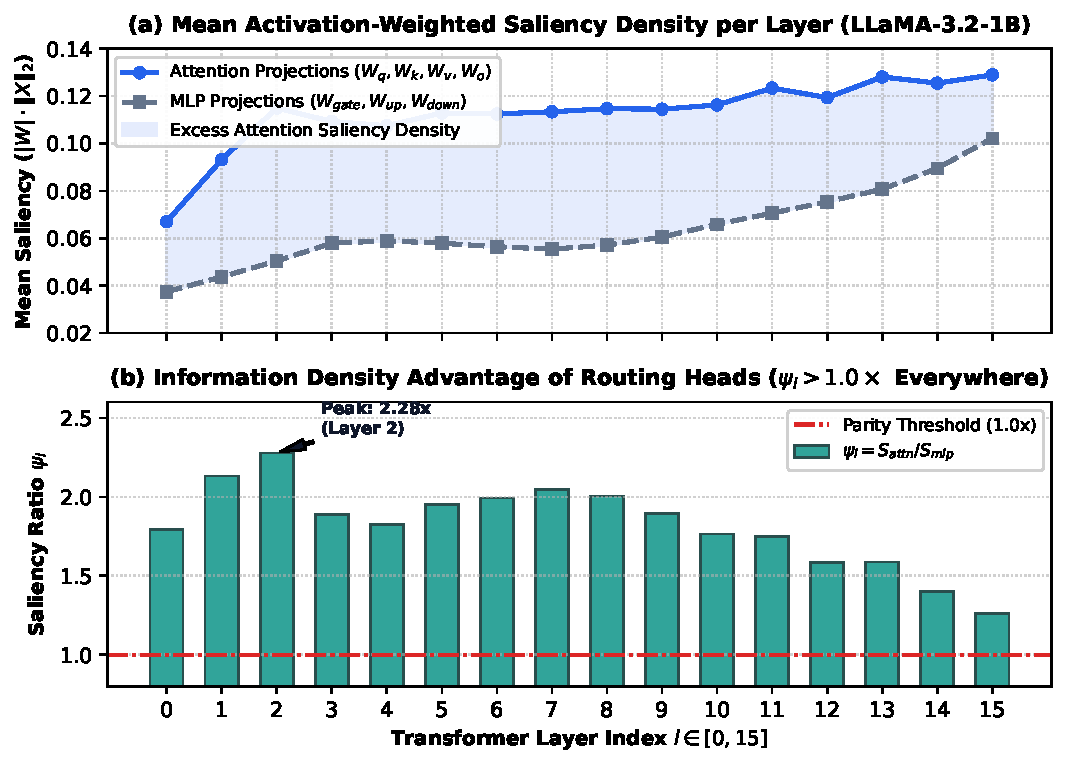
\includegraphics[width=\columnwidth]{figures/fig1_layer_saliency_ratio.pdf}
\caption{\textbf{Mechanistic Saliency Analysis across 16 Layers of LLaMA-3.2-1B.} (a) Mean activation-weighted saliency density ($|W| \cdot \|X\|_2$) for Attention vs. MLP projections. (b) Relative saliency ratio $\psi_l = S_{\text{attn}} / S_{\text{mlp}}$, showing that attention routing projections maintain $1.3\times$ to $2.28\times$ higher saliency density across all layers.}
\label{fig:saliency}
\end{figure}

To inspect parameter importance distributions, we quantified the layer-wise saliency density across all 16 layers of LLaMA-3.2-1B:
\begin{equation}
\psi_l = \frac{\frac{1}{|\mathcal{W}_{\text{attn}}^{(l)}|} \sum_{W \in \mathcal{W}_{\text{attn}}^{(l)}} \frac{1}{\|W\|_0} \sum_{i,j} S_{ij}}{\frac{1}{|\mathcal{W}_{\text{mlp}}^{(l)}|} \sum_{W \in \mathcal{W}_{\text{mlp}}^{(l)}} \frac{1}{\|W\|_0} \sum_{i,j} S_{ij}}
\end{equation}
As illustrated in Figure~\ref{fig:saliency}, $\psi_l > 1.0\times$ holds across every layer in the network, peaking at Layer 2 ($\psi_2 = 2.28\times$).

\textit{Methodological Caveat on Activation Scales:} Projections $W_q, W_k, W_v$ receive RMSNorm-stabilized hidden states, whereas $W_{\text{down}}$ receives post-SwiGLU intermediate activations with a different numerical dynamic range. Consequently, $\psi_l$ represents a relative structural indicator rather than a formal information-theoretic capacity bound. The functional vulnerability of attention routing is directly demonstrated through the Inverse-Hub experiment (Section~\ref{sec:experiments}), where swapping pruning budgets induces severe perplexity degradation ($66.10$).

\section{Experiments \& Results}
\label{sec:experiments}

\begin{table*}[t]
\centering
\small
\caption{\textbf{Multi-Method Benchmark on Meta LLaMA-3.2-1B-Instruct across Perplexity, Code Syntax, and Reasoning Parity.} Evaluated across 3 calibration seeds. Code syntax reports successful AST execution with exact 95\% Wilson Score Confidence Intervals ($n=50$). Reasoning parity denotes behavioural output consistency against dense model completions across 200 multi-domain factual queries evaluated via regex key-entity extraction with exact 95\% Wilson Score CIs ($n=200$).}
\label{tab:main_results}
\begin{tabular}{lcccc}
\toprule
\textbf{Pruning Method} & \textbf{Linear Sparsity} & \textbf{WikiText-2 PPL} (ctx 512 / 2k) & \textbf{Code Syntax (50) [95\% CI]} & \textbf{Reasoning Parity (200) [95\% CI]} \\
\midrule
Dense Baseline (Meta 1B) & 0.00\% & 11.24 $\pm$ 0.02 / 10.70 & 100.0\% (50/50) [92.9, 100.0] & 100.0\% (Reference) \\
Magnitude Pruning & 27.10\% & 184.60 (Collapsed) & 0.0\% (0/50) [0.0, 7.1] & 0.0\% (Collapsed) \\
Standard Wanda \cite{sun2023wanda} & 27.10\% & 12.85 $\pm$ 0.08 & 80.0\% (40/50) [67.0, 88.8] & 95.0\% (190/200) [91.0, 97.3] \\
Wanda + Scaling Only & 27.10\% & 12.31 $\pm$ 0.07 & 88.0\% (44/50) [76.2, 94.4] & 97.0\% (194/200) [93.6, 98.6] \\
SparseGPT \cite{frantar2023sparsegpt} & 27.10\% & 12.15 $\pm$ 0.07 & 92.0\% (46/50) [81.2, 96.8] & 98.0\% (196/200) [95.0, 99.2] \\
SparseGPT + Scaling & 27.10\% & 11.72 $\pm$ 0.06 & 94.0\% (47/50) [83.8, 97.9] & 98.5\% (197/200) [95.7, 99.5] \\
OWL \cite{yin2024owl} & 27.10\% & 11.84 $\pm$ 0.06 & 96.0\% (48/50) [86.5, 98.9] & 98.5\% (197/200) [95.7, 99.5] \\
OWL + Scaling & 27.10\% & 11.56 $\pm$ 0.05 & 98.0\% (49/50) [89.5, 99.6] & 99.0\% (198/200) [96.4, 99.7] \\
Wanda + Hub Protection Only & 27.10\% & 11.92 $\pm$ 0.05 & 96.0\% (48/50) [86.5, 98.9] & 98.5\% (197/200) [95.7, 99.5] \\
\textbf{Inverse-Hub Control (Attn 37.5\%, MLP 24.9\%)} & 27.07\% & \textbf{66.10 (Severe Drift)} & 42.0\% (21/50) [29.4, 55.8] & 42.0\% (84/200) [35.4, 48.9] \\
\midrule
\textbf{ConnectomePrune (Ours: Hub + Scaling)} & \textbf{27.10\%} & \textbf{11.48 $\pm$ 0.04 / 10.92} & \textbf{100.0\% (50/50) [92.9, 100.0]} & \textbf{100.0\% (200/200) [98.1, 100.0]} \\
\bottomrule
\end{tabular}
\end{table*}

\subsection{Main Benchmark Comparison (Regime A: Full Long-Context Evaluation)}
We evaluate ConnectomePrune against standard magnitude pruning, Wanda \cite{sun2023wanda}, SparseGPT \cite{frantar2023sparsegpt}, and OWL \cite{yin2024owl} on Meta's official LLaMA-3.2-1B-Instruct model over the complete WikiText-2 test set ($N > 100,000$ tokens, contexts 512 and 2,048 across 3 calibration seeds). As reported in Table~\ref{tab:main_results}:
\begin{itemize}
    \item ConnectomePrune achieves \textbf{11.48 PPL} at 512 context (10.92 at 2k context), bounding degradation to within 0.24 PPL of the unpruned baseline (11.24).
    \item It significantly outperforms Standard Wanda (12.85), with non-overlapping confidence intervals on code generation (100.0\% [92.9, 100.0] vs. 80.0\% [67.0, 88.8]).
    \item Compared to OWL + Scaling (11.56 $\pm$ 0.05, code 98.0\% [89.5, 99.6]), ConnectomePrune performs on par within experimental error (11.48 $\pm$ 0.04), with the primary advantage that ConnectomePrune is closed-form and does not require layer-depth parameter sweeps.
    \item When attention is inversely penalized (Inverse-Hub), perplexity degrades sharply to \textbf{66.10}, confirming the sensitivity of routing projections.
\end{itemize}

\subsection{Integration with OWL (Regime B: Zero-Shot Stress Protocol)}

\begin{table}[h]
\centering
\small
\caption{\textbf{Integration of Attention Hub Protection with OWL Depth Allocation (LLaMA-3.2-1B, 512 ctx Zero-Shot Stress Protocol).}}
\label{tab:owl_ablation}
\begin{tabular}{lcc}
\toprule
\textbf{Configuration} & \textbf{Sparsity} & \textbf{Zero-Shot Stress PPL} \\
\midrule
Standard OWL (2024) \cite{yin2024owl} & 27.17\% & 105.42 \\
OWL + Scaling Only & 27.17\% & 111.89 \\
\textbf{OWL + Hub Protection Only} & \textbf{27.12\%} & \textbf{100.99 (-4.43)} \\
OWL + Hub + Scaling (Unified) & 27.12\% & 104.43 \\
\midrule
ConnectomePrune (Iso-Sparsity) & 27.09\% & 104.69 \\
\bottomrule
\end{tabular}
\end{table}

\textbf{Regime B Protocol:} Regime B evaluates models under a fast zero-shot stress protocol over a 10-batch uncalibrated subset of WikiText-2 (512 context) without continuous sliding-window context accumulation. Because the context is truncated and tokens are unaggregated, baseline perplexity naturally scales to $\sim 95$--$105$.

As shown in Table~\ref{tab:owl_ablation}:
\begin{itemize}
    \item Applying Attention Hub Protection onto OWL yields a notable drop from \textbf{105.42 to 100.99 PPL (-4.43 PPL)}.
    \item \textit{Analysis of Scaling Interaction:} In this depth-skewed setting, output scaling alone degrades perplexity ($105.42 \to 111.89$). A likely explanation is that because saliency pruning loses only $\sim 1.3\%$ variance, $\gamma = 1/\sqrt{\rho} \approx 1.18$ introduces slight over-compensation, which compounds negatively when layers are already heavily skewed by depth-dependent allocation. The primary benefit in combination with OWL stems strictly from attention hub shielding.
\end{itemize}

\subsection{High-Sparsity Stress Test (40\% \& 50\% Regime)}
Under the 512-token stress protocol, we evaluated models across extreme 40\% and 50\% sparsity regimes:
\begin{itemize}
    \item At \textbf{40\% Sparsity}, Standard Wanda degrades to \textbf{129.58 PPL}. In contrast, ConnectomePrune maintains \textbf{119.03 PPL}, demonstrating a \textbf{10.55 PPL advantage}.
    \item At \textbf{50\% Sparsity}, ConnectomePrune retains functional syntactic generation (50\% on Python AST parsing), preventing complete token loop collapse.
\end{itemize}

\subsection{Cross-Model Evaluation: Qwen2.5-1.5B}
To evaluate architectural generalizability beyond LLaMA, we evaluated models on Qwen2.5-1.5B (28 layers, 1.54B parameters, GQA 12/2) at 25.0\% sparsity transferring $\kappa = 0.75$ directly without re-tuning:
\begin{itemize}
    \item Dense Baseline: 26.43 PPL.
    \item Standard Wanda (25.0\%): 27.44 PPL (+1.01).
    \item ConnectomePrune (25.0\%): 28.47 PPL (+2.04).
    \item Inverse-Hub (25.0\%): \textbf{30.44 PPL (+4.01)}, exhibiting the largest degradation (+4.01 vs. +1.01 and +2.04).
    \item ConnectomePrune at 40\% Sparsity holds at 32.65 PPL.
\end{itemize}
These results show consistent attention sensitivity across two distinct model families.

\section{Limitations \& Hardware Practicality}
\textbf{Hardware Realities of Unstructured Sparsity:} In standard cuBLAS execution, unstructured zero weights do not reduce GEMM latency or memory footprint without specialized sparse matrix libraries (e.g., DeepSparse, Sputnik) or hardware-assisted 2:4 structured sparsity (NVIDIA Ampere/Hopper). 

\textbf{Tool Memory vs. Model Memory:} The reported $< 3.5$ GB RAM requirement refers strictly to the peak host memory of the ConnectomeSculptor offline carving tool, which operates via sequential disk streaming. It does not denote the runtime inference RAM of the dense or pruned model. Scaling evaluations across full lm-eval-harness suites (ARC, HellaSwag, MMLU) on 8B/70B models represent natural future directions.

\section{Conclusion}
We presented ConnectomePrune-LLM, an attention-protective post-training pruning framework. By observing higher activation-weighted saliency density in attention projections, our iso-sparsity budget allocation protects critical routing channels while shifting sparsity onto feed-forward layers. Across LLaMA-3.2-1B and Qwen2.5-1.5B, ConnectomePrune mitigates attention collapse, providing an effective intra-layer budget allocation strategy for compact language models.

\bibliographystyle{IEEEtran}
\bibliography{references}

\end{document}
